
\begin{figure}
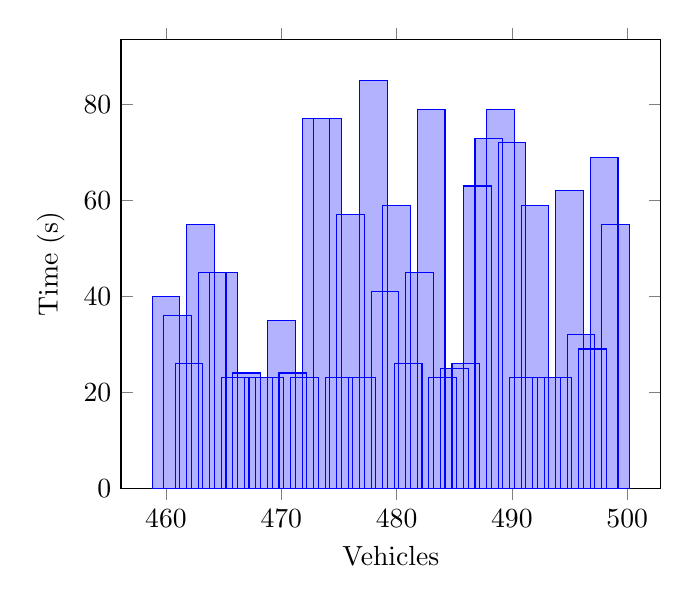
\begin{tikzpicture}
\begin{axis}[
legend style={anchor=west},
xlabel=Vehicles,
ylabel=Time (s),
ymin=0,
ybar,
]
\addplot coordinates {
(497, 29)
(499, 55)
(494, 23)
(495, 62)
(490, 72)
(491, 23)
(492, 59)
(493, 23)
(465, 45)
(460, 40)
(498, 69)
(496, 32)
(469, 23)
(464, 45)
(467, 24)
(461, 36)
(463, 55)
(462, 26)
(468, 23)
(466, 23)
(489, 79)
(488, 73)
(487, 63)
(486, 26)
(485, 25)
(484, 23)
(483, 79)
(482, 45)
(481, 26)
(480, 59)
(472, 23)
(473, 77)
(470, 35)
(471, 24)
(476, 57)
(477, 23)
(474, 77)
(475, 23)
(478, 85)
(479, 41)
};

\end{axis}
\end{tikzpicture}
\label{tik:time:100:15}
\caption{100 percent diving with GSC on route $15$}
\end{figure}
